\documentclass[11pt, a4paper]{article}
%\usepackage{proj1}
\usepackage{natbib}
\usepackage{fancyhdr}  
\usepackage{subcaption}
\usepackage{caption}
\usepackage{graphicx}
\usepackage{numprint}
\usepackage{multirow}
\linespread{1.25} 
\setlength{\parindent}{0cm}
\graphicspath{{Images/}}
\usepackage{hyperref}
\usepackage{amsmath}
\usepackage{amsfonts}
\usepackage{amssymb}
\usepackage{amsthm}
\usepackage{mathtools}
\usepackage{commath}
\usepackage{bbm}

%\usepackage[sc,osf]{mathpazo}
\usepackage{subcaption}
\usepackage[a4paper, top=1in, left=1.0in, right=1.0in, bottom=1in, includehead, includefoot]{geometry} %Usually have top as 1in

\usepackage{listings}
\usepackage{color} %red, green, blue, yellow, cyan, magenta, black, white
\definecolor{mygreen}{RGB}{28,172,0} % color values Red, Green, Blue
\definecolor{mylilas}{RGB}{170,55,241}


\hypersetup{colorlinks,linkcolor={black},citecolor={blue},urlcolor={black}}
\usepackage{color}
\urlstyle{same}


\theoremstyle{definition}
\newtheorem{definition}{Definition}[section]

\newcommand{\adja}{q_a}
\newcommand{\adjb}{q_b}
\newcommand{\adjaB}{q_{a,\partial \Omega}}
\newcommand{\adjbB}{q_{b,\partial \Omega}}
\newcommand{\adjB}{q_{\partial \Omega}}
\newcommand{\Adja}{\mathbf{p}}
\newcommand{\Adjb}{q}
\newcommand{\adj}{q}
\newcommand{\Adjc}{{q}_{\partial \Omega}}
\newcommand{\ra}{\rho_a}
\newcommand{\rb}{\rho_b}
\newcommand{\w}{\mathbf{w}}
\newcommand{\f}{\mathbf{f}}
\newcommand{\ve}{\mathbf{v}}
\newcommand{\n}{\mathbf{n}}
\newcommand{\h}{\mathbf{h}}
\newcommand{\K}{\mathbf{K}}
\newcommand{\hr}{\widehat \rho}
\newcommand{\jf}{\mathbf j}

%	\begin{figure}[h]
%		\centering
%		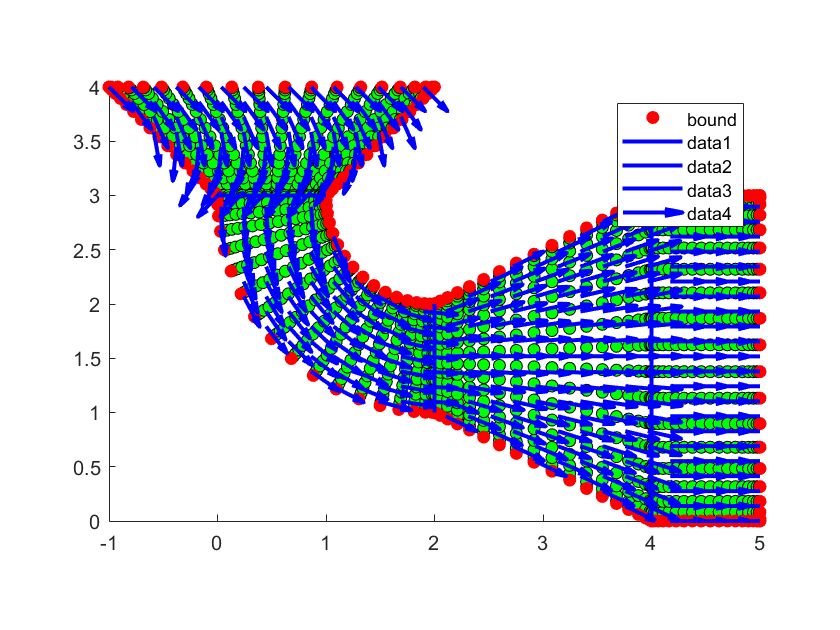
\includegraphics[scale=0.35]{F1.png}
%		\caption{Forward $\rho$ for $a = 0.01$} 
%		\label{F1}
%	\end{figure}

\begin{document}
\section*{MultiShape Theory}
The code library 2DChebClass, introduced in \cite{GoddardPseudospectralCode1}, is a tool for solving PDEs using pseudospectral methods in one and two dimensions on different domains, such as quadrilaterals, wedges and periodic boxes. The aim of this library is to provide a toolbox for solving DDFT in an efficient and user-friendly manner. This includes the automatic set-up of differentiation and convolution matrices, interpolation and integration vectors, as well as domain discretization using pseudospectral methods, identification of boundaries and application of boundary conditions. The library's features are thoroughly explained in \cite{GoddardPseudospectralCode1}.
\\
While the library supports solutions to PDEs on various single shapes, the method is now extended to compute the solution to a PDE on a complex domain, or multishape, which is composed of a number of quadrilaterals and wedges. The philosophy of this multishape code is to use the existing code library \cite{GoddardPseudospectralCode1}, which is designed to efficiently and accurately solve PDEs on individual shapes, to do the same on a multishape with minimal additional effort. 
\\
\\
The solution of a PDE on such a multishape domain is achieved by employing the spectral element method (SEM), by thinking of each of the shapes as the discretization elements of SEM.
This method is similar to the finite element method (FEM). FEM discretizes a domain into elements and computes the solution to a given PDE on each of those elements. Expansions of basis functions are used, which are low order polynomials, for interpolation on an equispaced grid. SEM follows the same philosophy but uses higher order basis functions such as Chebyshev or Lagrange polynomials and Chebyshev-Lobatto points on the interpolation grid on each element, as opposed to an equispaced grid, to avoid the Runge phenomenon. At the intersections between the elements, $C^0$ continuity is enforced. SEM was first introduced by Patera \cite{SEMPatera84} using  Chebyshev polynomials as basis functions and later adapted to Lagrange polynomials by Komatitsch and Vilotte \cite{SEMLagrange98}.
While this method is widely used to solve PDEs in their weak form, in this work the strong form of the PDE is considered, since this aligns best with the existing framework. (?!) Furthermore, instead of just requiring continuity of the solution at the intersection of two elements, the flux (or first derivatives) are also matched. 
\\
\\
In the multishape extension to 2DChebClass, a given PDE is solved on each shape individually, using the preexisting tools in the code library.
This is done simultaneously by stacking the differentiation matrices, integration and interpolation vectors for each shape on top of one another. The initial condition is also given as a stacked vector, containing the information for each shape. This stacking is done using a fixed order of the shapes specified by the user. 
For example, given a function $f$ on a domain $\Omega$ consisting of three shapes labeled $1,2,3$, the solutions on each shape $f_1$, $f_2$ and $f_3$ are stored as:
\begin{align*}
	f_\Omega = [f_1 | f_2 | f_3],
\end{align*}
and similarly, a differentiation matrix $D_\Omega$ is defined as:
\begin{align*}
	D_\Omega = [D_1 | D_2 | D_3],
\end{align*}
where the $D_i$, $i = 1, 2, 3$ are the differentiation matrices on each shape.
\\
The code automatically identifies the intersection boundaries between two shapes when setting up the multishape. The code loops through each face of each shape and compares the points of each face with all faces of the other shapes. It furthermore checks for the possibility that the points of two faces are the same but in reverse order. 
\\
Once the intersections between the neighboring shapes are identified, boundary conditions can be applied. There are currently two options, although the addition of further boundary conditions is straightforward. For a continuous solution on the multishape, both the solution to the PDE and the flux are matched at these intersection boundaries. Alternatively, hard walls between two shapes can be simulated easily, by applying a no-flux boundary condition at that intersection boundary. On boundaries which are on the outside of the multishape, different boundary conditions, such as no-flux and Dirichlet conditions, can be applied in the same way as for single shapes.
\\
\\
When no-flux boundary conditions are applied, a further subtlety is that information about the normal vectors to each outward boundary need to be computed. The existing code library already provides the set of normals for each shape. The multishape extension uses this, alongside the information of which boundaries of each shape are outward boundaries, and which intersect with other shapes, to find the outward normals of the multishape. The only part that needs to be treated with care are the points where two shapes intersect at an outward boundary, since these have two different normals at that intersection point. This is treated in the same way as corners of a single shape, by taking the average of the two normals given by the two faces that meet at the given corner. This is illustrated in Figure \ref{F1} (+++ not yet, why +++)
	\begin{figure}[h]
		\centering
		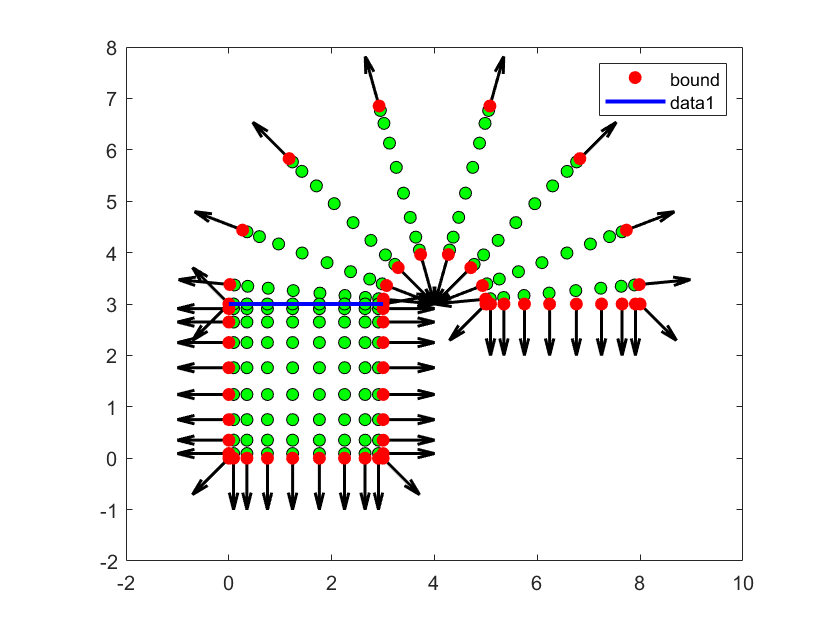
\includegraphics[scale=0.5]{normals.png}
		\caption{Needs fixing} 
		\label{F1}
	\end{figure}
\\
\\
The final aspect to be considered is the convolution matrix, which is needed to compute convolution integrals. It is computed in a similarly straightforward way, but since convolution is a global operation, it is not as simple as stacking the convolution matrices for the individual shapes, as is done for differentiation, integration and interpolation. 
The convolution integral is defined as:
\begin{align*}
	\left(n \star \chi \right) (y) = \int \chi (y - \tilde y) n (\tilde y) d \tilde y.
\end{align*}
As explained in \cite{GoddardPseudospectralCode1} in detail, $\chi$ at $y - \tilde y$ is evaluated for all points in the multishape domain and transformed into a matrix $\text{diag} \left(\chi\right)$. This is integrated, using the stacked integration vector, to result in the convolution matrix, which can then be applied to a density $n$.


\section{Validation Tests}
Several examples are run, using exact solutions, to test whether the multishape code works. This is done using an exact solution to the advection diffusion equation on an infinite domain, so that Dirichlet boundary conditions, matching the value of the exact solution on the boundary of the multishape, can be applied.
The exact solution is:
\begin{align*}
	\rho &= \exp(\alpha t + \beta_1 y_1 + \beta_2 y_2)\\
	\mathbf v &= \left(\beta_1 - \frac{\alpha}{2 \beta_1} + p_1\exp(-\beta_1 y_1) , \beta_2 - \frac{\alpha}{2 \beta_2} + p_2\exp(-\beta_2 y_2) \right),
\end{align*}
where $\beta_1 = -1$, $\beta_2 = 1$, $\alpha = 0.5$, $p_1 = -1$ and $p_2 = 1$.
At first, we compare the exact solution on a box of dimensions $[0,2] \times [0,2] $ with a multishape consisting of two boxes of dimensions $[0,2] \times [0,1]$ and $[0,2] \times [1,2]$, see Figure \ref{F2}. The question is whether the results of the PDE on the box and the dissected box are equal. Each of the shapes are discretized with $N = 20$ points in each spatial direction, which means that the dissected box has more points in total than the original box.
The relative error between the solutions on the two boxes is $1.0034 \times 10^{-10}$. 
When reducing the number of points in the dissected box to $N = 10$ per shape, while keeping $N = 20$ in the single shape box, the relative error in solution is $2.565 \times 10^{-10}$. The solution can be seen in Figure \ref{F3}.

	\begin{figure}[h]
		\centering
		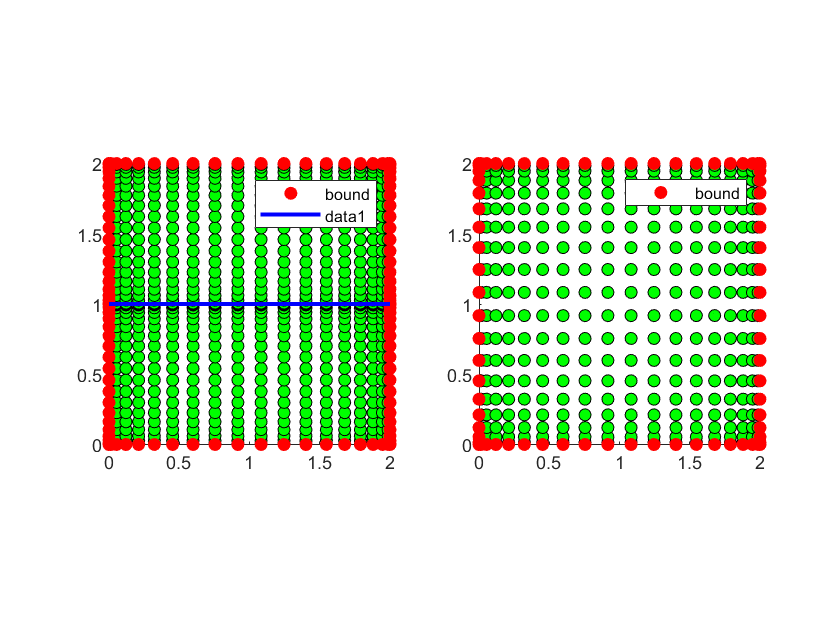
\includegraphics[scale=0.5]{disect1.png}
		\caption{The box and dissected box with $N = 20$} 
		\label{F2}
	\end{figure}

	\begin{figure}[h]
		\centering
		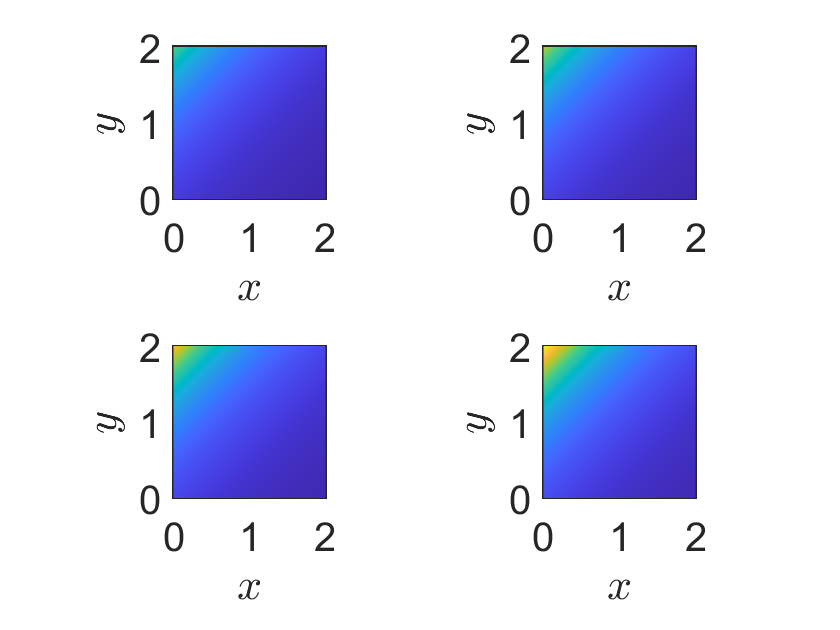
\includegraphics[scale=0.5]{disect2.png}
		\caption{Exact solution on the box} 
		\label{F3}
	\end{figure}
The same test can be done for a wedge. Here, a single wedge and a dissected version are considered, see Figure \ref{F4}. The error in solution between the two approaches with $N = 20$ is $2.0195 \times 10^{-7}$ and with $N = 10$ for each of the two shapes in the disected wedge and $N = 20$ in the full wedge the error is $3.349 \times 10^{-6}$. For $N = 30$ for the shapes in both domains the error is $9.8444 \times 10^{-11}$. This shows that the solution on the wedge is harder to compute accurately and needs more points as compared to the box. The solution can be seen in Figure \ref{F5}.
	\begin{figure}[h]
	\centering
	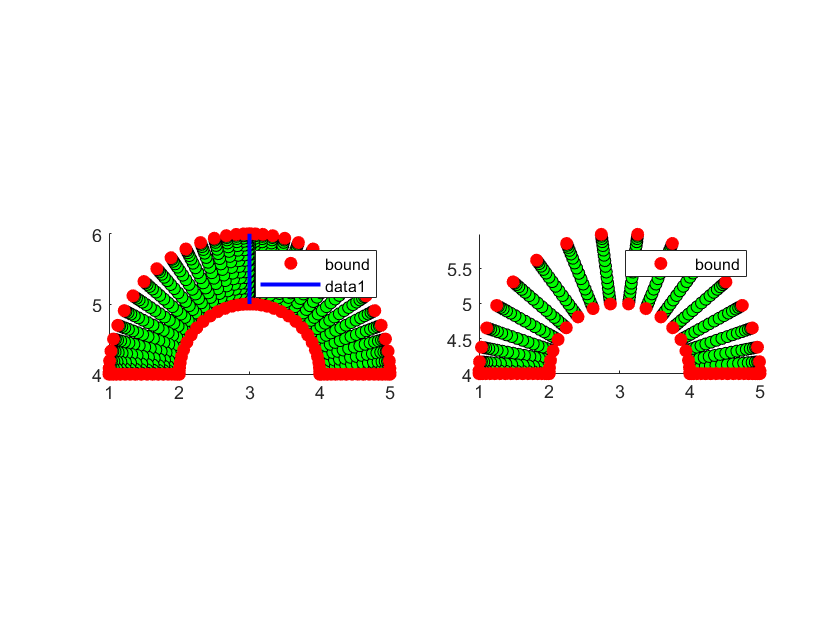
\includegraphics[scale=0.5]{disectW1.png}
	\caption{The wedge and dissected wedge with $N = 20$} 
	\label{F4}
\end{figure}

\begin{figure}[h]
	\centering
	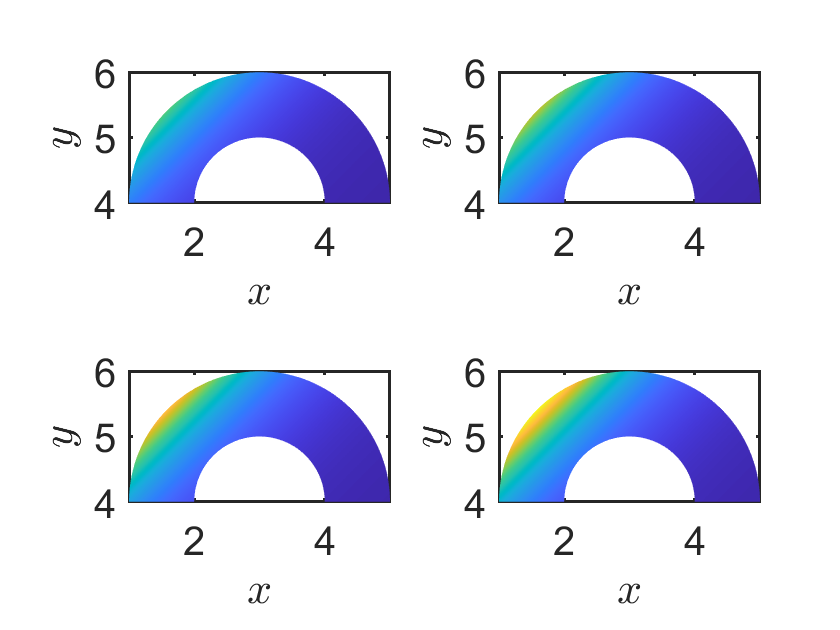
\includegraphics[scale=0.5]{disectW2.png}
	\caption{Exact solution on the wedge} 
	\label{F5}
\end{figure}

Next the advection diffusion equation is solved on a multishape which is composed of four quadrilaterals, see Figure \ref{F6}. The relative error for $N = 20$ on each shape as compared to the exact solution is $2.3321 \times 10^{-9}$. 
\begin{figure}[h]
	\centering
	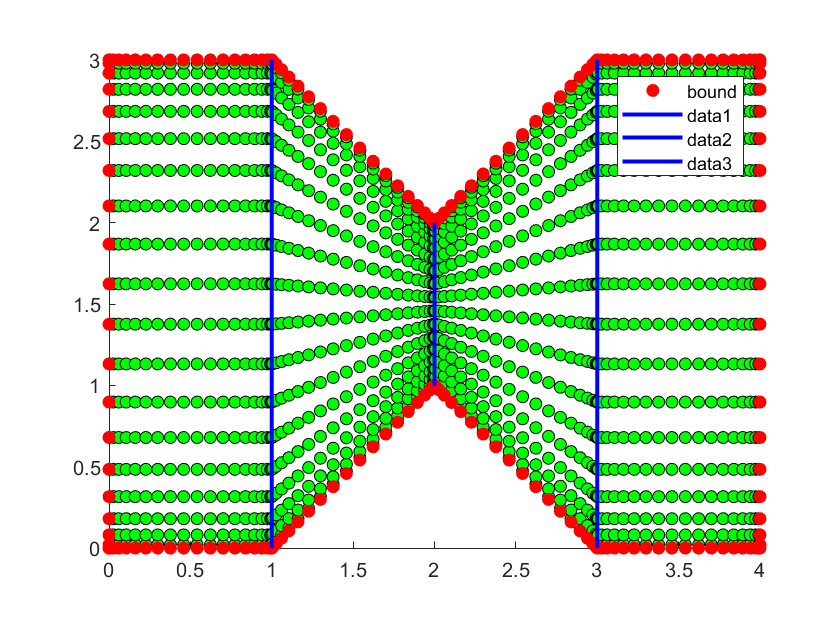
\includegraphics[scale=0.5]{example1.png}
	\caption{Example 1 multishape} 
	\label{F6}
\end{figure}
The same is done for a second example involving a wedge, see Figure \ref{F7}. The relative error to the exact solution is $1.3128 \times 10^{-7}$, when choosing $N= 20$ per shape. We again observe that a larger error is introduced when the multishape includes a wedge as compared to Example 1, which only included quadrilaterals. For $N = 30$ the error decreases to $2.2463 \times 10^{-9}$.

\begin{figure}[h]
	\centering
	\includegraphics[scale=0.5]{example2.png}
	\caption{Example 2 multishape} 
	\label{F7}
\end{figure}


\section{Forward Problems on multishapes}

The first example is solving an advection diffusion problem on a multishape consisting of two quadrilaterals and two wedges, with constant velocity of strength ten. The initial condition for this problem is:
 \begin{align*}
 	\rho_0 = \exp( -2(y_1 -0.5)^2 - 2 (y_2 + 1)^2).
 \end{align*}
The result, evaluated for $N= 20$ on each shape, can be seen in Figure \ref{F8}.

\begin{figure}[h]
	\centering
	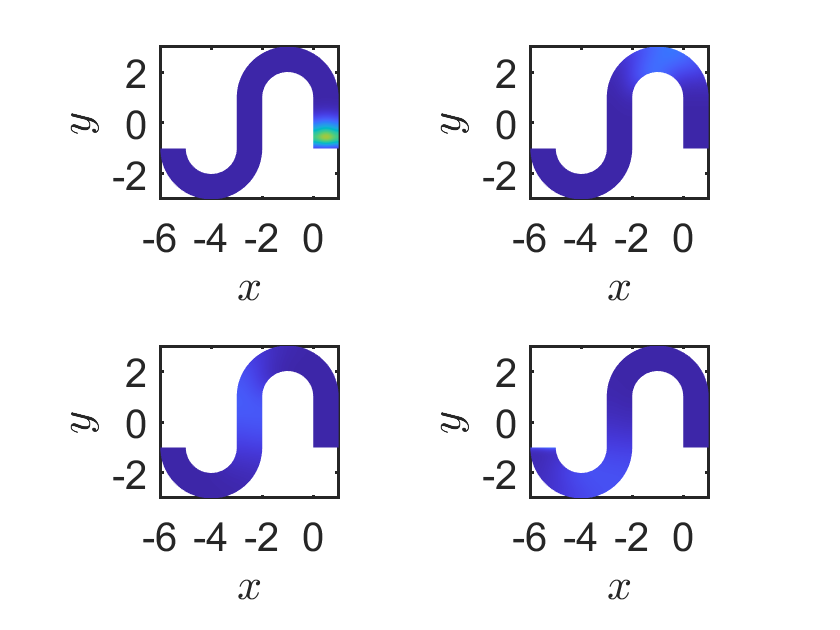
\includegraphics[scale=0.5]{ex1.png}
	\caption{Forward Problem 1}
	\label{F8}
\end{figure}

In a second example, the velocity is of strength $5$ and the initial condition is:
 \begin{align*}
	\rho_0 = \exp( -2(y_1 -0.5)^2 - 2 (y_2 - 1.5)^2).
\end{align*}
The result, which is computed on a multishape made up of four quadrilaterals into a channel, can be seen in Figure \ref{F9}.

\begin{figure}[h]
	\centering
	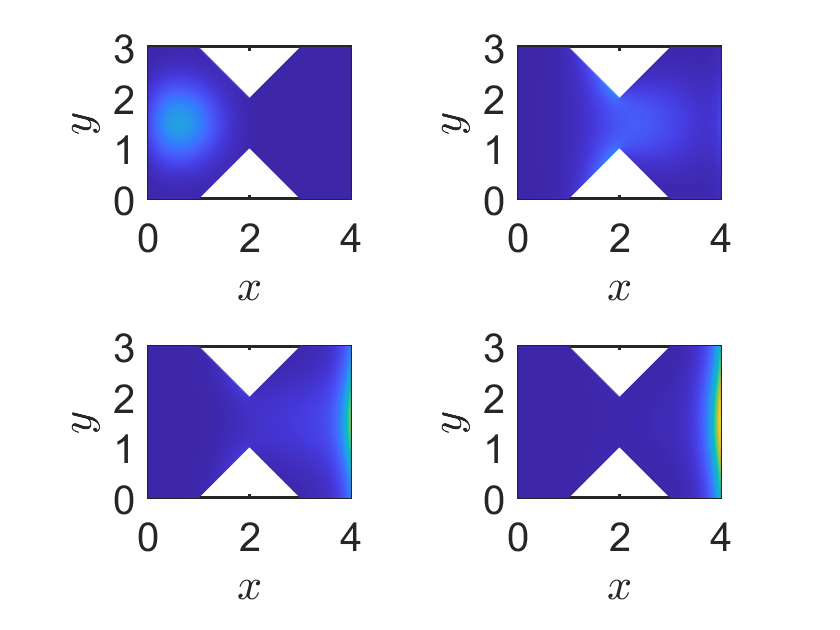
\includegraphics[scale=0.5]{ex2.png}
	\caption{Forward Problem 2}
	\label{F9}
\end{figure}








\pagebreak	
\bibliography{GeneralBib}
\bibliographystyle{unsrt}
\end{document}